\documentclass{ws-rv9x6}
\usepackage{ws-rv-thm}
\usepackage[square]{ws-rv-van}
\usepackage{simplewick}
\usepackage{relsize}
\usepackage{alphalph}

\newif\ifarxivsubmission

\arxivsubmissiontrue

\ifarxivsubmission
  \usepackage{color}
  \definecolor{darkblue}{rgb}{0.1,0.1,.7}
  \usepackage[colorlinks, linkcolor=darkblue, citecolor=darkblue, urlcolor=darkblue, linktocpage]{hyperref}
  \crop[off]{}
  \makeatletter
  \def\@makechapterhead#1{%                                                                                                      
    {\vbox to 110pt{%        %rvs                                                                                              
%   \refstepcounter{chapter}%                                                                                                  
    \def\thefootnote{\@fnsymbol\c@footnote}%                                                                                   
%   \addcontentsline{toc}{chapter}{\outchapter#1}                                                                              
    \vspace*{37pt}      %VSPACE FROM TRIM SIZE                                                                                 
        \parindent\z@\raggedright\reset@font
        {\centering{%{\CNfont Chapter~\thechapter\par}%                                                                         
         \vskip 0.25in
    \vbox{
    \CTfont #1\par
    }\par}\par}\nobreak\vfill}}}%  %rvs
  \makeatother
\else
  \usepackage[]{hyperref}
\fi

\makeindex

%\newcommand\be{\begin{eqnarray}}
%\newcommand\ee{\end{eqnarray}}
\def\be#1\ee{\begin{align}#1\end{align}}
\newcommand\f\phi
\newcommand\cO{\mathcal{O}}
\newcommand\p[1]{\left(#1\right)}
\newcommand\ptl\partial
\newcommand\e\epsilon
\newcommand\<\langle
\renewcommand\>\rangle
\newcommand\Z{\mathbb{Z}}
\newcommand\de\delta
\newcommand\R{\mathbb{R}}
\newcommand\bx{\mathbf{x}}
\newcommand\nn{\nonumber}
\renewcommand\.{\cdot}
\newcommand\x\times
\newcommand\pdr[2]{\frac{\partial #1}{\partial #2}}
\newcommand\s\sigma
\newcommand\SO{\mathrm{SO}}
\newcommand\De{\Delta}
\newcommand\cS{\mathcal{S}}
\newcommand\oo\infty
\newcommand\SU{\mathrm{SU}}
\newcommand\cH{\mathcal{H}}
\newcommand\bn{\mathbf{n}}
\newcommand\bP{\mathbf{P}}
\renewcommand\b\beta
\renewcommand\a\alpha
\newcommand\Tr{\mathrm{Tr}}
\renewcommand\l\lambda
\newcommand\cL{\mathcal{L}}
\newcommand\cD{\mathcal{D}}
\renewcommand\th{\theta}
\newcommand\tl[1]{\widetilde{#1}}
\newcommand\GeV{\mathrm{GeV}}
\newcommand\g\gamma
\newcommand\arXiv[1]{{\tt arXiv:#1}}
\newcommand\z\zeta
\renewcommand\hat[1]{\widehat{#1}}
\newcommand\bs{\mathbf{s}}
\newcommand\draftnote[1]{{\color{blue} #1}}

\newtheorem{exercise}{Exercise}[section]
\let\Exercisefont\itshape
\def\Exerciseheadfont{\bfseries}

\begin{document}

\ifarxivsubmission
\chapter{Phys 229ab Advanced Mathematical Methods:\ \ \\
Conformal Field Theory
}\label{ch:bootstrap}
\else
\chapter{The Conformal Bootstrap}
\fi

\author[David Simmons-Duffin]{David Simmons-Duffin}

\address{Caltech,
dsd@caltech.edu}

\begin{abstract}
Notes for Physics 229, 2017-2018. These notes are in progress. They were last updated on \today.
\end{abstract}
\body

\makeatletter
\newalphalph{\alphmult}[mult]{\@alph}{26}
\makeatother
\renewcommand{\thefootnote}{\alphmult{\value{footnote}}}

\ifarxivsubmission
  \thispagestyle{empty}
  \makeatletter
  \renewcommand*\l@chapter[2]{}
  \renewcommand*\l@schapter[2]{}
  \renewcommand*\l@author[2]{}
  \makeatother
  \newpage
  \setcounter{page}{1}
  \setcounter{tocdepth}{3}
  \smalltoc
  \tableofcontents
\fi

\ifarxivsubmission
  \newpage
\fi


\section{Introduction}

\subsection*{Resources}

These introductory notes are heavily based on Silviu Pufu's Bootstrap 2017 lectures \cite{} and John McGreevy's lectures on QFT \cite{}.

\subsection{QFT and emergent symmetry}

Quantum Field Theory is a universal language for theoretical physics. It shows up in many different settings, for example
\begin{itemize}
\item statistical physics,
\item condensed matter physics,
\item particle physics (SM and beyond),
\item string theory/holography.
\end{itemize}

The microscopic physics in all of these settings can be quite complicated. However, often the macroscopic physics displays extra ``emergent" symmetries that can help us do computations.

For example, in condensed matter physics, we are interested in describing a material made up of atoms with some lattice spacing $a$.\footnote{We ignore the possibility of lattice defects for the moment.} We refer to the detailed lattice system as the ``microscopic theory." Quantum field theory is a good description at distances much larger than the lattice spacing $x\gg a$, or equivalently energy/momenta much lower than the UV cutoff $\Lambda_{UV}=1/a$.\footnote{QFTs that are valid below a UV cutoff are often called ``effective field theories" (EFTs).} At these large scales, the discrete translation symmetry of the lattice becomes a continuous symmetry.

Similarly, in statistical physics, particle physics, and string theory, QFT can describe distance scales much larger than the characteristic scales of the microscopic theory.

Statistical systems are described by QFTs in Euclidean signature, e.g.\ on $\R^d$. Such QFTs capture properties of the equilibrium state. By contrast, condensed matter and particle systems are described by QFTs in Lorentzian signature, e.g.\ on $\R^{d-1,1}$. Such QFTs encode time-dependent quantum dynamics.

We will be interested in QFTs with rotational symmetry, by which we mean $\SO(d)$ symmetry in Euclidean signature and $\SO(d-1,1)$ symmetry in Lorentzian signature. In particle physics and string theory, this symmetry is built into the microscopic theory. However in lattice systems, rotational symmetry must be emergent. This means that correlation functions become rotationally invariant in the limit of large distances, even though microscopic correlation functions are not rotationally-invariant.\footnote{Emergent rotational symmetry is very familiar: we� often cannot determine the orientation of a microscopic lattice using macroscopic observations. Some examples of materials {\it without\/} emergent $\SO(d)$ symmetry are crystals like salt. A very exotic example is the Haah code \cite{}.} In particular, for condensed matter systems, the effective ``speed of light" associated with $\SO(d-1,1)$-invariance is an emergent property and has nothing to do with the speed of actual light. (We will see some explicit examples later.)

Under general conditions, $\SO(d)$-invariant Euclidean QFTs are in one-to-one correspondence with $\SO(d-1,1)$-invariant Lorentzian QFTs. The map between them is called Wick rotation, and we will discuss it in detail. Because of this correspondence, we can focus mostly on Euclidean QFTs, and later understand Lorentzian QFTs by Wick rotating what we learned in Euclidean signature.

\subsection{The mass gap and critical points}

So far, we are interested in theories with Poincare symmetry
\be
G_\mathrm{Poincare} &= \R^d \rtimes \SO(d).
\ee
From the point of view of long-distance physics, the most important property of a Poincare-invariant theory is its mass gap 
\be
m_\mathrm{gap} &= E_1-E_0,
\ee
where $E_0,E_1$ are the energies of the ground state and first excited state, respectively.\footnote{Some QFTs with topological order can have multiple degenerate ground states.} Theories with $m_\mathrm{gap}>0$ are called ``gapped." 

To understand why $m_\mathrm{gap}$ is important, let us study a two-point function of a scalar local operator $\f(x)=\f(x^0,\mathbf{x})$. We  demand that $\f(0)$ have vanishing vacuum expectation value by subtracting off an appropriate multiple of the unit operator. By Poincare invariance, it suffices to consider $\<0|\f(x^0,\mathbf{0}) \f(0)|0\>$ with $x^0>0$. The two-point function is then given by
\be
\<0|\f(x^0,\mathbf{0})\f(0)|0\> &= \<0|\f(0) e^{-H x^0} \f(0)|0\> \nn\\
&= \sum_\psi |\<0|\f(0)|\psi\>|^2 e^{-E_\psi x^0}.
\ee
Here, $H$ is the Hamiltonian with the vacuum energy subtracted off, and $\psi$ runs over an orthonormal basis of eigenstates of $H$. To get the right-hand side, we have used $\f(x^0,\mathbf{0}) = e^{H x^0} \f(0,\mathbf{0}) e^{-H x^0}$ and  $H|0\>=0$.\footnote{Note that the Euclidean time-evolution operator is $e^{-H x^0}$ as opposed to the familiar $e^{-iHt}$ in Lorentzian signature. They are related by Wick rotation $x^0 = i t$. We will discuss this in much more detail in later sections.}

The key point is that the operator $e^{-H x^0}$ exponentially damps states with energy $E_\psi\gg 1/x^0$.
 %%We have the Kallen-Lehmann spectral representation
%%\be
%%\<\f(x)\f(y)\> &= \int dm^2 \rho(m^2) G_F(x-y,m),
%%\ee
%%where $G_F(x,m^2)$ is the Feynman propagator with mass $m$. Here, $\rho(m^2)\geq 0$ is an effective density of states with mass $m$. If we demand that $\f(0)$ have vanishing vacuum expectation value (by subtracting off an appropriate multiple of the unit operator), then the support of $\rho(m^2)$ is contained in $[m_\mathrm{gap}^2,\oo)$.
%%
%% For simplicity, consider $d=3$ where the Feynman propagator simplifies
%%\be
%%G_F(x,m) &= \frac{1}{4\pi |x|} e^{-m|x|} \qquad (d=3).
%%\ee
%The key point is that $G_F(x,m)$ falls off exponentially as $e^{-m|x|}$ in Euclidean signature. At large $|x|$, the two-point function is then dominated by contributions with the smallest $m$, and thus falls off as $e^{-m_\mathrm{gap} |x|}/|x|$ if $m_\mathrm{gap}$ is nonzero.\footnote{It could fall faster if the operator $\f(x)$ has zero amplitude to create the lightest state in the theory.}
%
%A more general way to see the exponential falloff is to write the two-point function as
%\be
%\<0|\f(x^0,\mathbf{0}) \f(0)|0\> &= \<0|\f(0)e^{-H x^0} \f(0)|0\>,
%\ee
%where $H$ is the Hamiltonian (with the ground state energy subtracted off), and we have taken the points to be separated only in the $x^0$ direction for simplicity.\footnote{Note that in Euclidean theories, the time-evolution operator is $e^{-H x^0}$ as opposed to $e^{-iHt}$ familiar from quantum mechanics. We will discuss this in much more detail later in the course.} 
At large $x^0$, the correlator is dominated by $\psi$ with the smallest nonzero eigenvalue of $H$, which is $m_\mathrm{gap}$.\footnote{Note that the vacuum does not contribute as an intermediate state because we have demanded $\<0|\f(0)|0\>=0$.)}

Thus, when $m_\mathrm{gap}$ is nonzero, correlation functions of local operators fall off at least as fast as $e^{-|x|/\xi}$, where $\xi\equiv 1/m_\mathrm{gap}$ is called the ``correlation length." Generic statistical and condensed matter systems have microscopic correlation lengths $\xi \sim a$, or equivalently $m_\mathrm{gap} \sim \Lambda_{UV}$. At long distances, they are described by QFTs whose local correlation functions vanish, called topological quantum field theories (TQFTs).

%Generic statistical and condensed-matter systems are gapped. In such systems, correlations at scales $x\gg \l$ are effectively zero.\footnote{Gapped theories are described by topological quantum field theories (TQFTs) and are interesting in their own right. However, we will not focus on TQFTs in this course.}

 However, sometimes by tuning parameters in the microscopic Hamiltonian, we can make $m_\mathrm{gap}$ much smaller than $\Lambda_{UV}$, and even arrange for $m_\mathrm{gap}$ to vanish. Points in parameter space where $m_\mathrm{gap}=0$ are called critical points.
At a critical point, the system experiences a phase transition, and develops nonzero correlations at arbitrarily long distances.\footnote{If the Standard Model were like a generic condensed matter system, we might expect $m_\mathrm{gap}$ to be close to the UV cutoff, which is perhaps the GUT scale $10^{15}\GeV$ or Planck scale $10^{18}\GeV$. The hierarchy problem is the problem of explaining why the Standard Model is so close to a critical point.}

Long-distance correlation functions at critical points have no intrinsic length-scale because all memory of dimensionful microscopic quantities (like the lattice spacing $a$) disappears when distances become arbitrarily large. For example, critical two-point functions behave as pure power laws
\be
\<\f(x)\f(0)\> &= \frac{C}{|x|^{2\De}} \qquad(\textrm{critical point, }x\gg a),
\ee
where $C$ and $\De$ are constants depending on $\phi$. The quantity $\De$ is called the scaling dimension of $\f$.

\subsection{Scaling and conformal symmetry}

A more precise way to state the lack of an intrinsic length scale is to say that theories with $m_\mathrm{gap}=0$ have an emergent symmetry under rescaling
\be
\label{eq:rescalingsymmetry}
x^\mu \to \l x^\mu\qquad (\l>0).
\ee
Under very general conditions (that we will discuss), critical points also display less obvious emergent symmetries called conformal transformations. A conformal transformation $x\to x'(x)$ is a map that looks like a rotation and rescaling near each point,
\be
\pdr{x'^\mu}{x^\nu} &= \Omega(x) R^{\mu}{}_\nu(x),\qquad R^{\mu}{}_\nu\in \SO(d).
\ee
An example is a special conformal transformation,
%a less-obvious emergent symmetry under special conformal transformations
\be
\label{eq:specialconformalsymmetry}
x^\mu \to \frac{x^\mu - b^\mu x^2}{1-2 b\.x + b^2 x^2}\qquad(b\in \R^d).
\ee
In 2-dimensions, there are more exotic examples, like the one pictured in figure~\ref{}.\footnote{We will give a precise definition for what it means for a theory to be invariant under transformations like (\ref{eq:rescalingsymmetry}) and (\ref{eq:specialconformalsymmetry}) later in the course.}

Here is some rough intuition for why critical points display conformal symmetry. We know that a critical theory is invariant under rescalings and rotations. If the theory is also local, in the sense that degrees of freedom at a point only interact directly with other degrees of freedom at nearby points, then the theory should also be invariant under transformations that locally look like a rescaling and rotation. This is the defining property of a conformal transformation. Turning this rough intuition into a theorem is a difficult problem (that we will discuss in more detail later). However, it seems to be true in a wide class of systems.

QFTs that are invariant under conformal symmetry are called conformal field theories (CFTs). To summarize, CFTs describe critical points where $m_\mathrm{gap}=0$. One can also understand the neighborhood of a critical point where $m_\mathrm{gap}$ is nonzero (but still $m_\mathrm{gap} \ll \Lambda_{UV}$) by studying perturbations of the associated CFT.

\subsection{Examples of critical points}

So far our discussion has been very abstract, so let us introduce some examples. 
%Through examples, we will try to explain
%\begin{itemize}
%\item Why statistical systems are described by Euclidean QFT,
%\item How different microscopic theories are described by the same CFT (universality),
%\item How to tune $m_\mathrm{gap}\to 0$ in a solvable model,
%\item How to study (some) CFTs using conventional QFT tools like perturbation theory.
%\end{itemize}
One of our goals will be to infer from examples a set of axioms that CFTs should satisfy. We will study these axioms in the next part of the course. Another goal will be to be more precise about how and why statistical and condensed matter systems are described by quantum field theory, and how critical points come about.

\subsubsection{Magnets}

Our first examples of critical points occur in magnets. Given a magnet with temperature $T$, we can apply a magnetic field $\vec{H}$ and measure the magnetization $\vec{M}$. There are three main types of magnets in 3-dimensions, which are distinguished by their symmetries:\footnote{Here, we mean non-spacetime symmetries, usually called ``global" or ``flavor" symmetries. The emergent spacetime symmetry group is still the Poincare group, or the conformal group at the critical point.}
\begin{itemize}
\item {\it Uni-axial magnet}: individual magnetic moments $\vec\mu$ are confined to lie along a fixed axis. Uni-axial magnets have an $O(1)=\Z_2$ symmetry under which $\vec H \to -\vec H$ and $\vec M \to -\vec M$.

\item {\it XY magnet}: magnetic moments $\vec\mu$ are oriented in a plane. Such magnets have an $O(2)$ symmetry under which $\vec H$ and $\vec M$ rotate in the plane.

\item {\it Heisenberg magnet}: magnetic moments $\vec \mu$ are unconstrained. Such magnets have $O(3)$ symmetry under which $\vec H$ and $\vec M$ transform in the vector representation.
\end{itemize}
For the moment, we will focus on the simplest case of uni-axial magnets. We denote the projections of $\vec H,\vec M$ onto the appropriate axis by $H,M$.

In experiments, we observe the following. There exists a ``critical temperature" $T_c$, such that
\begin{itemize}
\item For $T<T_c$, the preferred state of the magnet has nonzero magnetization $M\neq 0$ when $H=0$. In other words, the $\Z_2$ symmetry is spontaneously broken.
\item For $T>T_c$, the magnet has $M=0$ when $H=0$, i.e.\ the $\Z_2$ symmetry is unbroken.
\end{itemize}
The corresponding phase diagram is pictured in figure~\ref{}. The point 
\be
H = 0,\ T=T_c
\ee
is a critical point, and is described by a CFT at long distances. To reach the critical point, we must tune two parameters: $H$ and $T$. Tuning $H=0$ is easy because that is where the microscopic theory has $\Z_2$ symmetry. However, the value of $T_c$ depends on the specific material.

In more detail, the behavior of the magnetization in different phases is shown in figure~\ref{}. Close to $T_c$, observables exhibit so-called ``scaling" behavior, characterized by various critical exponents. Let us define the dimensionless couplings 
\be
\label{eq:dimensionlesscouplings}
t \equiv \frac{T-T_c}{T_c},\qquad h=\frac{H}{k_B T}.
\ee
Some examples of critical exponents are
\begin{itemize}
\item $\a$: the heat capacity at $h=0$ behaves as
\be
C &= \frac{\ptl^2 F}{\ptl T^2} \propto |t|^{-\a}.
\ee
(Here $F$ is the free-energy.)

\item $\b$: the spontaneous magnetization behaves as
\be
\lim_{H\to 0^+} M &\propto (-t)^\b.
\ee

\item $\gamma$: the zero-field susceptibility behaves as
\be
\chi &= \left.\pdr{M}{H}\right|_{H=0} \propto |t|^{-\g}.
\ee

\item $\de$: the magnetization at $T=T_c$ behaves as
\be
|M|&\propto|h|^{1/\de}.
\ee

\item $\nu$ and $\eta$: the correlation length $\xi$ can be measured by studying a two-point correlation functions of spins 
\be
G(x) &= \<s(x)s(0)\> - \<s(0)\>^2.
\ee
Away from the critical point, $G(x)\sim e^{-|x|/\xi}$ decays exponentially. However, as $t\to 0$, the correlation length diverges as
\be
\xi &\propto |t|^{-\nu}.
\ee
Equivalently, the mass-gap goes to zero as $m_\mathrm{gap}\propto |t|^\nu$.
Precisely at $t=0$, the two-point function takes the form
\be
G(x) &\propto \frac{1}{|x|^{d-2+\eta}},
\ee
i.e.\ the spin operator has dimension $\Delta_s = \frac{d-2}{2}+\frac \eta 2$.
\end{itemize}

Don't worry, I can't keep track of all these critical exponents either. We will see shortly that all of this behavior can be explained using effective field theory, scaling symmetry, and dimensional analysis.

Now, here is an amazing fact:
\begin{claim}
We find the same critical exponents in many different uni-axial magnets, regardless of what material they're made of.
\end{claim}
In fact, critical uni-axial magnets are all described by the same scale-invariant QFT at long distances. This phenomenon is called ``critical universality."

\subsubsection{Liquid-vapor transitions}

Other critical points appear in liquid-vapor transitions. For example, the phase-diagram of water is pictured in figure~\ref{}. Near room temperatures and pressures, there is a sharp distinction between the liquid and gas phases. However, at  higher temperatures and pressures, the distinction between liquid and gas disappears at a critical point $(T_c,P_c)$.  For example, in water $T_c=647\,\mathrm{K}$, $P_c=374\,\mathrm{Atm}$.

Note that the critical points of magnets and water are both obtained by tuning two parameters. Comparing neighborhoods of the critical points in figures~\ref{} and \ref{}, we can make the following rough analogy between water and magnets:
\be
P-P_c &\sim H, \nn\\
\rho-\rho_c &\sim M.
\ee
where $\rho$ is the density and $\rho_c$ is the critical density.\footnote{Water does not have a microscopic $\Z_2$ symmetry, but it turns out that one emerges near the critical point. Roughly speaking, the $\Z_2$ switches the liquid (high-density) and gas (low-density) phases. To make a more precise analogy, we should identify $M$ with the combination of $\rho$ and $P$ that flips sign under the emergent $\Z_2$.}

In measurements of critical water, we again observe scaling behavior. For example, the heat capacity behaves as
\be
C &\sim |t|^{-\a},
\ee
where $t$ is again given by (\ref{eq:dimensionlesscouplings}).
Additionally, the difference in density between the liquid and gas phases behaves as
\be
\rho_\mathrm{liquid}-\rho_\mathrm{gas} &\sim (-t)^\b.
\ee
Amazingly,
\begin{claim}
Water and other liquid-vapor transitions have precisely the same critical exponents as uni-axial magnets.
\end{claim}
We say that liquid-vapor transitions are in the same ``universality class" as uni-axial magnets.

\hfill \draftnote{\it End of lecture 1}

\subsubsection{The Ising model}

The Ising model is a simplified model of a magnet that is still rich enough to capture its critical behavior. Its degrees of freedom are classical spins taking values $\pm 1$, with one spin for each site on a cubic lattice\footnote{The Ising model can also be formulated on other lattices, and in many cases these models lie in the same universality class.}
\be
s_i \in \{\pm 1\},\qquad i \in \Z^d.
\ee
The partition function is a sum over all configurations of spins, with Boltzmann weights that mimic the interactions between physical spins in a magnet,
\be
Z(K,h) &= \sum_{\{s_i\}} e^{-S[s]}, \nn\\
S[s] &= -K \sum_{\<ij\>} s_i s_j - h \sum_j s_j.
\ee
The notation $\<ij\>$ means that $i,j$ are neighboring lattice sites. (You can think of $K$ as the product $\b J$ where $\b$ is the inverse temperature and $J$ is the spin-spin interaction.) We can also compute correlation functions by inserting spins into the sum
\be
\<s_{i_1} \cdots s_{i_n}\> &= \frac{1}{Z}\sum_{\{s_i\}} s_{i_1} \cdots s_{i_n} e^{-S[s]}.
\ee
The ``magnetization" is proportional to the one-point function $\<s_i\>$ (which is independent of $i$).

When $K$ is positive, the term in $S[s]$ proportional to $K$ makes spins want to align. This term has a $\Z_2$ symmetry under which $s_i\to -s_i$ for all $i$. The term proportional to $h$ breaks this $\Z_2$ symmetry and causes spins to preferentially have the same sign as $h$. Both of these effects compete against statistical fluctuations.

In dimension $d \geq 2$, the Ising model famously exhibits a critical point at a special value $K=K_c$ and $h=0$. For $K>K_c$, spins spontaneously align and break the $\Z_2$ symmetry. For $K<K_c$, statistical fluctuations cause the spins to randomize and the $\Z_2$ is unbroken.

The Ising critical point displays precisely the same long-distance correlation functions and critical exponents as real uni-axial magnets and liquid-vapor systems. In fact, for our purposes, we can think of the Ising model as yet another physical system in the same universality class as these other systems. Its main distinguishing feature is that it is much simpler than e.g.\ actual water, and thus much easier to study.\footnote{There are many other abstract statistical lattice models in the same universality class as the Ising model, for example compass models \arXiv{1303.5922} and the Blume-Capel model \arXiv{1711.10946}. The Ising model on a cubic lattice is arguably the simplest, however the Blume-Capel model has some features that make it even better for simulation.} By studying the mathematics of the Ising model, we will be able to understand gaplessness and a few QFT/CFT axioms in a simple way. By the power of critical universality, quantities we compute in the abstract Ising model at $K=K_c$ agree exactly with interesting quantities in real physical systems.

\subsubsection{Continuum $\f^4$ theory}

The Ising lattice model is a good starting point for understanding why classical statistical systems are described by QFT at long distances. We can think of each configuration of spins as a map
\be
s: \Z^d \to \{\pm 1\},
\ee
and the partition function is a sum over all such maps. This is a discrete version of a path integral.

Typically, in QFT we integrate over continuous functions on a continuous space, e.g.\ 
\be
\f : \R^d \to \R.
\ee
If we study correlation functions of the Ising model at long distances (much larger than the lattice spacing), it's not hard to imagine that we can approximate the lattice as continuous $i\in\Z^d \to x\in\R^d$. Similarly, we can replace individual spins $s_i$ with average densities of spins $\f(x)$ in small neighborhoods, so that the effective spin at a point becomes a real number. 

This suggests that the partition sum of the Ising model might be related to the path integral for a scalar field on $\R^d$, at least at long distances. That is, perhaps we can take
\be
\Z^d &\to \R^d\nn\\
s_i &\to \phi(x) \nn\\
\sum_{\{s_i\}} &\to \int D\phi \nn\\
e^{-S[s]} &\to e^{-S[\phi]},
\ee
for some continuum action $S[\f]$, without changing the long-distance behavior of correlation functions too much.

There is a non-rigorous procedure called ``taking the continuum limit" of a lattice model that tries to justify these replacements. However, it involves several uncontrolled approximations, and it is perhaps more honest to just study a continuum scalar theory and compare its behavior with the Ising model.

For concreteness, let us focus on 3-dimensions. The simplest interacting theory of a scalar field in 3d has Euclidean action
\be
\label{eq:continuumphifour}
S[\f] &= \int d^3 x \p{\frac 1 2 (\ptl \phi)^2 + \frac 1 2 m^2 \f^2 + g \f^4}.
\ee
Note that $\f$ has mass-dimension $1/2$, so that $m$ and $g$ both have mass-dimension $1$. Thus, $\f^2$ and $\f^4$ are relevant interactions, and we can think of this theory as an RG flow from the free-boson at high energies to something else at low energies.

Let us map out the phase diagram of this theory. Because $m$ and $g$ are the only dimensionful parameters, only their ratio matters.\footnote{To be more precise, there is also a UV cutoff $\Lambda$ that depends on how the theory is regularized. The quartic term gives rise to a linear divergence proportional to the $\f^2$ term, so  physical masses are given by $m_\mathrm{phys}^2 = m^2 + \a g \Lambda$, with $\a$ a dimensionless number. (In some regularization schemes, like dimensional regularization, the linear divergence vanishes.) However, shifting $m^2$ is the only way the cutoff can enter a physical observable. Thus, our discussion becomes correct after the replacement $m^2 \to m^2_\mathrm{phys}$.}   Suppose first that $m^2/g^2 \gg 0$ is large and positive. In this limit, the theory has a single massive vacuum with mass approximately $m_\mathrm{gap} \approx m$. Now suppose $m^2/g^2 \ll 0$ is very negative. In this case, the theory has two very massive vacuua that spontaneously break the $\Z_2$ symmetry, with $m_\mathrm{gap}\approx \sqrt {-2m^2}$.

If we start at very large $|m^2|$ (in either phase) and decrease $|m^2|$, $m_\mathrm{gap}$ decreases too. There exists a critical ratio $m^2/g^2 = r_c$ where $m_\mathrm{gap}\to 0$ and the theory is described by a nontrivial CFT. One can justify this claim using the $\e$-expansion and other perturbative techniques, as we will discuss, or from numerical simulations.

The phase diagram we have just described is the same as the Ising phase diagram. Indeed $\f^4$-theory is also in the Ising universality class.

Near the critical point, the $\f^4$ interaction cannot be treated as a small perturbation. More explicitly, because the coupling constant $g$ has mass-dimension 1, perturbation theory is really an expansion in $g x$, where $x$ is the characteristic length scale of the observable we are computing. In the long-distance limit $x\to \oo$ (where the CFT emerges), this expansion breaks down. Thus, the Ising CFT cannot be studied with traditional perturbation theory. We will later discuss two different perturbative (but uncontrolled) expansions for the Ising CFT: the $\e$-expansion and the large-$N$ expansion.

\begin{figure}
\begin{center}
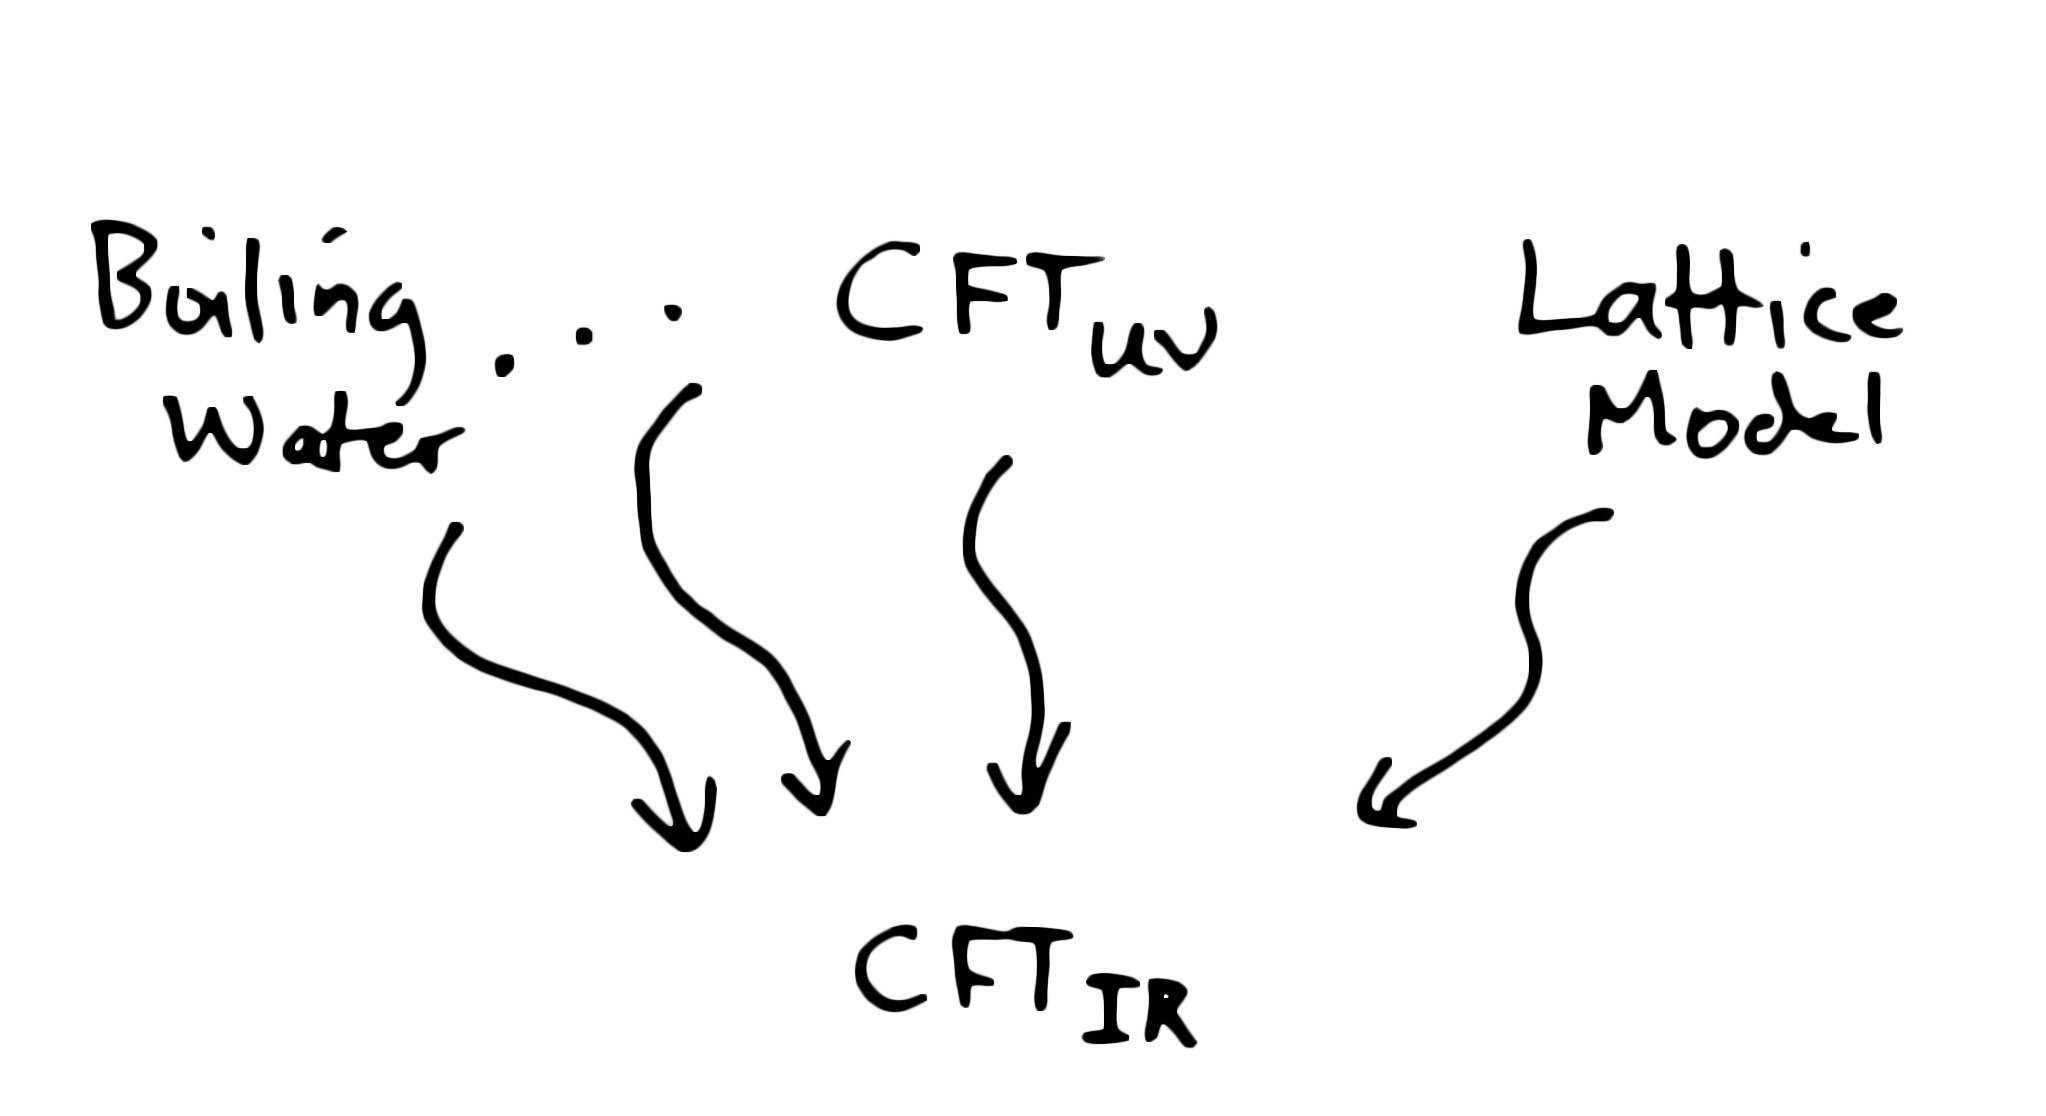
\includegraphics[width=0.55\textwidth]{rgflows-ising.jpg}
\end{center}
\caption{Many  microscopic theories can flow to the same IR CFT\@. We say that the theories are IR equivalent, or IR dual. \label{fig:rgflows}}
\end{figure}

The theory with action (\ref{eq:continuumphifour}) and $m^2/g^2=r_c$ is equivalent to the free boson at short distances (high energies/UV) and the Ising CFT at long distances (low energies/IR). The free boson is itself a CFT, so we have an RG flow from one CFT to another (figure \ref{fig:rgflows}). This construction, where we start with a UV CFT and  perturb it so that it flows to an IR CFT, is one possible definition of a general QFT. In this definition, we must allow for the possibility that the IR theory is gapped, in which case $\mathrm{CFT}_\mathrm{IR}$ is a TQFT which is technically a special case of a CFT (where all local correlation functions are zero).

An RG flow from the free boson is perhaps the cleanest theoretical construction of the Ising CFT. It shows that the Ising CFT inherits properties of a continuum quantum field theory. For example, $\f^4$-theory has rotational invariance and $\Z_2$ symmetry, so the Ising CFT does too. The Ising lattice model is easier to simulate, but it does not have microscopic rotational symmetry. Meanwhile, water has rotational symmetry but no microscopic $\Z_2$ symmetry. We will learn a lot about the Ising CFT by going back and forth between different microscopic realizations.

\subsubsection{Other universality classes}

We have seen several different systems that fall into the Ising universality class. However, not every critical point is described by the Ising CFT. Another important class of 3d CFTs are the $O(N)$ models. These can be described as the critical point of a theory of $N$ bosons $\f_i$ ($i=1,\dots,N$) with a quartic interaction that respects an $O(N)$ global symmetry
\be
S &= \int d^3 x \p{\frac 1 2 \sum_i \ptl_\mu \f_i \ptl^\mu \f_i + \frac 1 2 m^2 \sum_i \f_i \f_i + g \p{\sum_i \f_i \f_i}^2}.
\ee
XY magnets are in the same universality class of the $O(2)$ model and Heisenberg magnets are in the same universality class of the $O(3)$ model.

But this is just the tip of the iceberg --- there is a huge zoo of different types of critical points that we can construct in a variety of ways. One of our goals will be to better understand this zoo.

\section{Path integrals, quantization, and the quantum-classical correspondence}

In this section, we explain in more detail why classical statistical systems are described by Euclidean quantum field theory, and also how they are related to quantum condensed-matter systems via Wick rotation. Along the way, we will introduce some important technical concepts in QFT, like cutting-and-gluing rules for path integrals and the idea of quantization. This section is heavily based on John McGreevy's lectures \cite{}.

\subsection{The 1d Ising model and the transfer matrix}

Let us start with the Ising lattice model in 1-dimension. For concreteness, we will study the theory on a periodic lattice with length $M$, so the spins $s_i$ are labeled by $i\in \Z_M$.  The partition function is given by
\be
Z_1 &= \sum_{\{s_i=\pm 1\}} e^{-S[s]} \nn\\
S[s] &= -K \sum_{i=1}^{M} s_i s_{i+1} - h \sum_{i=1}^M s_i.
\ee
We refer to $S[s]$ as the ``action," even though it is equal to $\b H$, where $H$ is the classical Hamiltonian. This is because we would like to reserve the word Hamiltonian for a completely different object that will appear shortly.

As mentioned in the introduction, the partition sum should be thought of as a discrete version of a 1-dimensional path-integral. This 1-dimensional path integral can be computed by relating it to a 0-dimensional quantum theory. This is an example of the notion of {\it quantization}.

The key idea is to build up the partition sum by moving along the lattice site-by-site. Forget about periodicity for the moment, and consider the contribution to the partition function from spins $j<i$ for some fixed $i$,
\be
Z_\mathrm{partial}(i,s_i) &= \sum_{\{s_j:j<i\}} e^{K\sum_{j < i} s_j s_{j+1} + h \sum_{j< i} s_j}.
\ee
Because of the interaction term $s_{i-1}s_{i}$, we cannot do the sum over $\{s_1,\dots, s_{i-1}\}$ without specifying the spin $s_i$. Thus, we have a function of $s_i$. In short, $Z_\mathrm{partial}(i,s)$ is the partition function of the theory on the lattice $1\dots i$, with fixed boundary condition $s$ at site $i$.\footnote{We must also impose some boundary condition at site $1$. The precise choice is not important for this discussion, so we have left it implicit.}

Note that $Z_\mathrm{partial}(i+1,s_{i+1})$ can be related to $Z_\mathrm{partial}(i,s_{i})$ by inserting the remaining Boltzmann weights that depend on $s_i$ and performing the sum over $s_i=\pm 1$,
\be
\label{eq:onestepsum}
Z_\mathrm{partial}(i+1,s_{i+1}) &= \sum_{s_i = \pm 1} T(s_{i+1},s_i) Z_\mathrm{partial}(i,s_{i}),
\ee
where
\be
T(s_{i+1},s_i) &\equiv e^{K s_i s_{i+1} + h s_i}.
\ee

The key step is to recognize (\ref{eq:onestepsum}) as a discrete version of the Schrodinger equation in a 2-dimensional Hilbert space $\mathcal{H}$. This Hilbert space has basis $|s\>=|\pm 1\>$. The $T(s',s)$'s are elements of a $2\x 2$  matrix $\hat{T}$ acting  on $\mathcal{H}$
%We can think of $T(s',s)$ as elements of a $2\x 2$ matrix and $Z_\mathrm{partial}(s)$ as components of a vector in a 2-dimensional Hilbert space,
\be
T(s',s) &= \<s'|\hat{T}|s\>,\qquad \hat{T} =
\begin{pmatrix}
e^{K+h} & e^{-K-h} \\
e^{-K+h} & e^{K-h}
\end{pmatrix},
\ee
and $Z_\mathrm{partial}(i,s)$ are the components of a vector $|\Psi_i\>\in \mathcal{H}$,
\be
Z_\mathrm{partial}(i,s) &= \<s|\Psi_i\>.
\ee
In this notation, (\ref{eq:onestepsum}) becomes
\be
\label{eq:discreteshrodinger}
|\Psi_{i+1}\> &= \hat{T} |\Psi_i\>.
\ee
The matrix $\hat{T}$ is called the ``transfer matrix", and it plays the role of a discrete time-translation operator. Here, $i$ should be thought of as a discrete Euclidean time coordinate.

To be explicit, the (integrated) Schrodinger equation in a quantum theory in Euclidean time is
\be
|\Psi(\tau+\Delta\tau)\> &= e^{-\De\tau \hat H} |\Psi(\tau)\>,
\ee
where $\tau$ is the Euclidean time coordinate, $\De\tau$ is some time-step, and $\hat H$ is the quantum Hamiltonian. Thus,  the $1$-dimensional Ising lattice model is equivalent to a 2-state quantum theory with Hamiltonian
\be
\hat H &= -\frac{1}{\Delta\tau} \log \hat T.
\ee

When the lattice is periodic, the partition function is related to the transfer matrix by
\be
\label{eq:partitionfunctionastransfermatrix}
Z_1 %&= \sum_{\{s_i\}} T(s_M, s_{M-1}) T(s_{M-1},s_{M-2}) \cdots T(s_1,s_M) \nn\\
&= \sum_{\{s_i\}} \<s_M|\hat{T}|s_{M-1}\>\<s_{M-1}|\hat{T}|s_{M-2}\> \cdots \< s_1|\hat{T}|s_M\> \nn\\
&= \Tr(\hat{T}^M).
\ee
This is now easy to evaluate by diagonalizing $\hat T$,
\be
\Tr(\hat{T}^M) &= \l_+^M + \l_-^M,
\ee
where
\be
\l_\pm &= e^K \cosh h \pm \sqrt{e^{2K} \sinh^2 h + e^{-2K}} \nn\\
&\to \begin{cases}
2\cosh K \\
2\sinh K
\end{cases}\qquad (\textrm{when }h=0).
\ee

In the thermodynamic limit $M\to\oo$, the partition function is dominated by the larger eigenvalue
\be
Z_1 &=\l_+^M \p{1+\p{\frac{\l_-}{\l_+}}^M} \approx \l_+^M.
\ee
In quantum mechanical language, the state with the largest eigenvalue of $\hat T$ has the smallest eigenvalue of $\hat H$ --- i.e.\ it is the ground state, and we should call it $|0\>$. We have shown that the ground state dominates the thermodynamic limit. Contributions from the excited state are exponentially suppressed in the energy gap times the size of the system
\be
\p{\frac{\l_-}{\l_+}}^M &= e^{-(M\Delta\tau) m_\mathrm{gap}}, \nn\\
m_\mathrm{gap} &\equiv - \frac 1 {\Delta \tau} \log (\l_-/\l_+).
\ee

\hfill \draftnote{\it End of lecture 2}

We can also use the transfer matrix to compute correlation functions. For example, consider the two-point function $\<s_{i_1} s_{i_2}\>_{\Z_M}$ where the subscript $M$ indicates that we are on a periodic lattice with length $M$. Suppose $i_1>i_2$. We have
\be
\<s_{i_1} s_{i_2} \>_{\Z_M} &= \frac 1 {Z_1} \sum_{\{s_i\}} \<s_M|\hat{T}|s_{M-1}\> \cdots \<s_{i_1+1}|\hat{T}|s_{i_1}\> s_{i_1} \<s_{i_1}|\hat{T}|s_{i_1-1}\>\cdots \nn\\
& \qquad \x\cdots\<s_{i_2+1}|\hat{T}|s_{i_2}\> s_{i_2} \<s_{i_2}|\hat{T}|s_{i_2-1}\>\cdots \<s_1|\hat{T}|s_M\> \nn\\
&= \frac{1}{Z_1}\Tr(\hat{T}^{M-i_1} \hat{\s}^z \hat{T}^{i_1 - i_2}\s^z \hat T^{i_2}) \qquad (i_1 > i_2).
\label{eq:correlatorastrace}
\ee
Here, we introduced the Pauli spin operator $\s^z$ that measures the spin of a state
\be
\s^z|s\> &= s|s\>.
\ee
It is easy to compute the correlation function (\ref{eq:correlatorastrace}) by expressing $\hat s$ in the eigenbasis of $\hat T$.
\begin{exercise}
Show that in the limit of large $M$ and large ``distance" $i_1-i_2$, the correlator factorizes into a product of expectation values $\<0|\s^z|0\>$, plus exponential corrections from the excited state
\be
\<s_{i_1} s_{i_2}\>_{\Z_M} &= \<0|\s^z|0\>^2 + O(e^{-m_\mathrm{gap} \tau}, e^{- m_\mathrm{gap}(L-\tau)}),
\ee
where $\tau\equiv (i_1-i_2)\Delta\tau$, $L\equiv M\Delta\tau$.
\end{exercise}

Let us write (\ref{eq:correlatorastrace}) in a slightly different way by introducing ``Heisenberg picture" operators
\be
\hat s(i) &= \hat T^{-i} \s^z \hat T^i.
\ee
Equation~(\ref{eq:correlatorastrace}) is equivalent to
\be
\label{eq:heisenbergtwopt}
\<s_{i_1} s_{i_2}\>_{\Z_M} &= \frac 1 {Z_1} \Tr(\hat s(i_1) \hat s(i_2) \hat T^M) \qquad (i_1 > i_2).
\ee
Note that in deriving (\ref{eq:correlatorastrace}, \ref{eq:heisenbergtwopt}), we used that $i_1>i_2$. If instead $i_2 > i_1$, the path integral would give a product of operators in the opposite order
\be
\<s_{i_1} s_{i_2}\>_{\Z_M} &= \frac 1 {Z_1} \Tr(\hat s(i_2) \hat s(i_1) \hat T^M ) \qquad (i_2 > i_1).
\ee
The general statement is that the path integral becomes a time-ordered product of quantum operators\footnote{We hope that the time-ordering symbol $T\{\cdots\}$ will not be confused with the transfer matrix.}
\be
\label{eq:periodiccorrelationlattice}
\<s_{i_1} \cdots s_{i_n}\>_{\Z_M} &= \frac{1}{Z_1}\Tr(T\{ \hat s(i_1) \cdots \hat s(i_n)\}\hat T^M ),
\ee
where the definition of the time-ordering symbol is
\be
T\{\hat s (i_1)\cdots \hat s(i_n)\} &\equiv \hat s(i_1)\cdots \hat s(i_n) \theta(i_1 > \cdots > i_n) + \mathrm{permutations}.
\ee
Here $\theta(i_1 > \cdots > i_n)$ is $1$ if the $i_k$ are in the specified order and zero otherwise.

Finally, in the limit of large-$M$, the factor $\frac{\hat T^M}{\l_+^M}$ projects onto the ground state, so a path integral on the full lattice $\Z$ becomes a vacuum expectation value of a time-ordered product
\be
\label{eq:fulllattice}
\<s_{i_1}\cdots s_{i_n}\>_\Z &= \<0|T\{ \hat s(i_1) \cdots \hat s(i_n)\}|0\>.
\ee

\begin{exercise}
Consider adding a next-to-nearest neighbor interaction to the 1d Ising model
\be
S[s] &= \sum_{i} K s_{i}s_{i+1} + K' s_{i} s_{i+2}.
\ee
Find the associated quantum Hilbert space and transfer matrix, and compute the partition function on $\Z_M$ in the limit of large $M$.
\end{exercise}

\subsection{Quantization in quantum mechanics}

The procedure of turning a path integral into a product of quantum operators is called quantization. It is an extremely general procedure that ultimately stems from ``cutting and gluing" rules of the path integral.

For a more familiar example, let us review quantization for the path integral of a quantum particle on the real line. This theory has Euclidean action
\be
S[x] &= \int d\tau \p{\frac 1 2 \dot x^2 + V(x)},
\ee
where $x(\tau)$ is a map from Euclidean time $\tau$ to $\R$.
%To quantize, we introduce an orthonormal basis state $|x\>$ for every classical configuration at a fixed time $\tau_0$. These are the analogs of $|s=\pm 1\>$ in the Ising case, which were in one-to-one correspondence with classical configurations at a fixed lattice site $i_0$.
Consider the path integral on the interval $\tau\in[\tau_a,\tau_b]$ with fixed boundary conditions
\be
\label{eq:qmtransitionamplitude}
U(x_b,\tau_b;x_a,\tau_a) &\equiv \int_{\substack{x(\tau_b)=x_b \\ x(\tau_a) = x_a}} Dx(\tau) e^{-S[x]}.
\ee
By grouping paths according to their positions at a fixed time $\tau_c\in(\tau_a,\tau_b)$, we obtain a simple ``gluing" rule for $U$,
\be
\label{eq:gluingruleqm}
U(x_b,\tau_b;x_a,\tau_a) &= \int_{-\oo}^\oo dx_c U(x_b,\tau_b;x_c,\tau_c)U(x_c,\tau_c;x_a,\tau_a).
\ee

To quantize the theory, we build up the path integral  in small time-increments using the gluing rule. Suppose we have already computed the path integral $U(x_0,\tau_0;x_a,\tau_a)$ on the interval $[\tau_a,\tau_0]$. To extend $\tau_0\to \tau_0+\e$, we write
\be
\label{eq:gluingforsmallinterval}
U(x_1,\tau_0+\e;x_a,\tau_a) &= \int dx_0\, U(x',\tau_0+\e;x_0,\tau_0) U(x_0,\tau_0;x_a,\tau_a).
\ee
The quantity
\be
U(x_1,\tau_0+\e;x_0,\tau_0) &= U(x_1,\e;x_0,0).
\ee
plays the role of a transfer matrix, and $U(x_0,\tau_0;x_a,\tau_a)$ plays the role of a state at time $\tau_0$. To see this, we introduce a Hilbert space
\be
\label{eq:qmhilberspace}
\mathcal{H} &= \mathrm{Span}\{|x\> : x\in \R\}
\ee
with inner product $\<x'|x\>=\de(x-x')$.
The $|x\>$ are analogs of the basis states $|s=\pm 1\>$ in the Ising model. Defining $\hat T_\e$ and $|\Psi(\tau_0)\>$ by
\be
\<x_1|\hat T_\e|x_0\> &= U(x_1,\e;x_0,0),\nn\\
\<x_0|\Psi(\tau_0)\> &= U(x_0,\tau_0;x_a,\tau_a),
\ee
equation (\ref{eq:gluingforsmallinterval}) becomes
\be
\label{eq:transfermatrixforqmeq}
|\Psi(\tau_0+\e)\> &= \hat T_\e |\Psi(\tau_0)\>.
\ee

To recover the Schrodinger equation, we must show that 
\be
\hat T_\e &= 1 - \e \hat H + O(\e^2),
\ee
where
\be
\hat H &= -\frac 1 2 \frac{\ptl^2}{\ptl x^2} + V(x)
\ee
is the usual quantum-mechanical Hamiltonian. This is a standard argument, and we give a quick version here for completeness. We have
\be
\<x_1|\hat T_\e|x_0\> &= \int_{\substack{x(\e)=x_1 \\ x(0) = x_0}} Dx(\tau) e^{-S[x]},\qquad(\e \ll 1)\nn\\
S[x] &= \int_0^\e d\tau \p{\frac 1 2 \dot x^2 + V(x)}.
\ee
Because the time interval is so short, if $|x(\tau)-x_0|$ ever becomes larger than $O(\e)$, the kinetic term will cause the amplitude to be highly suppressed. Thus, let us assume $|x(\tau)-x_0|$ is of order $\e$. This means we can replace $V(x)\to V(x_0)$ (up to subleading corrections in $\e$), so the potential factors out of the integrand
\be
e^{-S[x]} &= e^{-\e V(x_0)} \exp\p{\int_0^\e d\tau \frac{\dot x^2}{2}}.
\ee

We can now split $x(\tau)$ into a classical term and a fluctuation term $\z(\tau)$ with boundary conditions $\z(0)=\z(\e)=0$,
\be
x(\tau) &= x_0\p{1-\frac{\tau}{\e}} + x_1\frac{\tau}{\e} + \z(\tau),\nn\\
\int_0^\e d\tau \frac{\dot x^2}{2} &= \frac{(x_1-x_0)}{2\e} + \int_0^\e d\tau \frac{\dot\z^2}{2}.
\ee
The path integral over $\z$ contributes a constant $A_\e$ that depends on how the theory is regulated.\footnote{A very simple regulator is to approximate $x(\tau)$ as a piecewise linear path with segments of length $\e$. This is equivalent to simply setting $\z=0$ and not doing the integral.} We thus find
\be
\<x_1|\hat T|x_0\> &= A_\e e^{-\e V(x_0)} e^{-\frac{(x_1-x_0)^2}{2\e}}(1+O(\e)).
\ee
Finally, the Gaussian factor can be expanded in $\e$ using
\be
\label{eq:simplifyexponential}
e^{-\frac{x^2}{2\e}} &= \sqrt{2\pi \e}\p{\de(x) + \frac \e 2 \de''(x) + O(\e^2)},
\ee
which gives
\be
\<x_1|\hat T|x_0\> &= A_\e \sqrt{2\pi \e} \p{\de(x_1-x_0) - \e\p{-\frac 1 2\de''(x_1-x_0) + V(x_0)\de(x_1-x_0)} + O(\e^2)} \nn\\
 &= A_\e \sqrt{2\pi \e}\<x_1|1 - \e \hat H + O(\e^2)|x_0\>.
\ee
The prefactor $A_\e \sqrt{2\pi \e}$ is an overall regulator-dependent constant that can be renormalized away by adding a ``cosmological constant" term to the action.

Thus, in the limit $\e\to 0$, equation (\ref{eq:transfermatrixforqmeq}) becomes a Euclidean version of the Schrodinger equation
\be
\frac{d}{d\tau} |\Psi(\tau)\> &= - \hat H|\Psi(\tau)\>.
\ee
Integrating using the initial condition $U(x',0,x,0)=\de(x-x')$, we find
\be
\label{eq:pathintegralwithbcsasamplitude}
U(x_b,\tau_b;x_a,\tau_a) &= \<x_b|e^{-\hat H (\tau_b-\tau_a)} |x_b\>.
\ee

Path integrals on different geometries correspond to different quantum mechanical observables. For example, the path integral on a circle $S^1_\b$ of length $\b$ with periodic boundary conditions is equal to
\be
\int_{-\oo}^\oo dx\, U(x,\b;x,0) = \Tr(e^{-\b \hat H}),
\ee
which is the quantum partition function at inverse temperature $\b$.
This is the continuum analog of equation~(\ref{eq:partitionfunctionastransfermatrix}).
Inserting observables into the path integral gives a time-ordered product of the associated quantum operators. For example, with periodic boundary conditions,
\be
\label{eq:periodiccorrelation}
\<x(\tau_1) \cdots x(\tau_n)\>_{S^1_\b} &=
\int_{x(\b)=x(0)} Dx\, x(\tau_1) \cdots x(\tau_n) e^{-S[x]}\nn\\
 &= \Tr(T\{\hat x(\tau_1) \cdots \hat x(\tau_n)\} e^{-\b \hat H}),
\ee
where we introduced the operator
\be
\hat x(\tau) &= e^{\tau \hat H} \hat x e^{-\tau \hat H}, \nn\\
\hat x|x\> &= x|x\>.
\ee
To derive (\ref{eq:periodiccorrelation}), we cut the interval $[0,\b]$ into segments $[0,\tau_1]\cup [\tau_1,\tau_2] \cup \cdots [\tau_n,\b]$ (assuming $\tau_n > \cdots > \tau_1$) and use (\ref{eq:pathintegralwithbcsasamplitude}) for each segment.
The operator $\hat x$ is the analog of $\hat s$ and equation~(\ref{eq:periodiccorrelation}) is the analog of (\ref{eq:periodiccorrelationlattice}).

Finally, in the limit $\b\to \oo$, the factor $e^{-\b \hat H}$ projects onto the ground state. Thus the Euclidean path integral on $\R$ is equal to a time-ordered correlation function in the ground state,
\be
\<x(\tau_1) \cdots x(\tau_n)\>_{\R} &= \<0|T\{\hat x(\tau_1) \cdots \hat x(\tau_n)\}|0\>.
\ee
This is the continuum analog of (\ref{eq:fulllattice}).

\hfill \draftnote{\it End of lecture 3}

\subsection{The 2d Ising model}

Let us now consider a slightly more complicated case: the 2d Ising model. This will be a good toy example for how cutting, gluing, and quantization work in a general QFT. For simplicity, we set $h=0$. We consider the partition function on the doubly-periodic lattice $\Z_{M} \x \Z_{N}$ and label spins $s_{i,j}$ by a pair $(i,j) \in \Z_{M} \x \Z_{N}$.

The action is given by
\be
S[s] &= -K\sum_{i,j} (s_{i,j}s_{i+1,j}  +  s_{i,j}s_{i,j+1}) \nn\\
&= K \sum_{i,j} \p{\frac 1 2 (s_{i,j+1} - s_{i,j})^2 - 1} - K \sum_{i,j}  s_{i,j} s_{i+1,j} \nn\\
&= \mathrm{const.} + \sum_{j=1}^{N} L( \bs_{j+1}, \bs_{j}).
\label{eq:unimportant}
\ee
In the last line, we split the action into contributions from pairs of neighboring rows.
The notation $s_{j}$ represents the configuration of spins in the $j$-th row,
\be
(\bs_{j})_{i} &= s_{i,j}.
\ee
The action associated with a pair of neighboring rows is given by
\be
L(\bs',\bs) &= \frac 1 2 K \sum_{i=1}^{M}(\bs'_i - \bs_i)^2 - \frac 1 2 K \sum_{i=1}^{M}(\bs_{i+1} \bs_i + \bs'_{i+1} \bs'_i).
\ee
(The constant in (\ref{eq:unimportant}) gives an unimportant multiplicative constant in the path integral that will disappear in normalized correlation functions, so we will ignore it.)

To quantize the theory, we can think of the $j$ direction as time, so $s_{j}$ is interpreted as a classical configuration on a fixed time-slice. The Hilbert space has an orthonormal basis vector for each such configuration,
\be
\label{eq:twodisinghilbert}
\mathcal{H}_{M} &= \mathrm{Span}\left\{|\pm\! 1, \pm 1, \cdots,\pm 1\>\right\} \nn\\
&= \bigotimes_{i=1}^{M} \mathcal{H}_i,
\ee
where $\mathcal{H}_i$ is a 1-qubit Hilbert space for each site $i$. $\mathcal{H}_{M}$ is the quantum Hilbert space of $M$ qubits, and is $2^{M}$-dimensional.

The transfer matrix between successive time slices is a $2^{M} \x 2^{M}$ matrix with entries
\be
\<\bs'|\hat T|\bs\> &= e^{-L(\bs',\bs)}.
\ee
The partition function on $\Z_{M} \x \Z_{N}$ is then
\be
\label{eq:partitionfunctionastracetwod}
Z(\Z_{M} \x \Z_{N}) &= \Tr_{\mathcal{H}_{M}}(\hat T^{N}).
\ee
To compute correlation functions, we need an operator that measures the spin at site $i$. This is simply the Pauli spin matrix $\s^z_i$ associated with the $i$-th site
\be
\s^z_i |s_1,\dots,s_j,\dots,s_{M}\> &= s_i |s_1,\dots,s_i,\dots,s_{M}\>.
\ee
We also have Heisenberg picture operators
\be
\label{eq:oldspinop}
\hat s_{i,j} &= \hat T^{-j} \s_i^z \hat T^j.
\ee
Correlation functions become traces of time-ordered products, e.g.
\be
\<s_{i_1,j_1} s_{i_2,j_2}\> &= \Tr_{\mathcal{H}_{M}}(\hat T^{N+j_2-j_1} \s_{i_1}^z \hat T_2^{j_1-j_2} \s_{i_2}^z) \th (j_1-j_2) + (1\leftrightarrow 2) \nn\\
&= \Tr_{\mathcal{H}_M}(T\{\hat s_{i_1,j_1} \hat s_{i_2,j_2}\} \hat T^{N}).
\ee

Let us now emphasize an important new ingredient in the 2-dimensional case compared to the 1-dimensional case. To arrive at (\ref{eq:partitionfunctionastracetwod}), we had to choose $j$ as the time direction. We then cut the path integral along rows of constant $j$. However, we could just as well have chosen $i$ as the time direction and cut the path integral along columns of constant $i$. This would give a different Hilbert space $\mathcal{H}_N$ with dimension $2^N$, a new transfer matrix $\hat T'$ (acting on $\mathcal{H}_N$), and a different formula for the same path integral,
\be
Z(\Z_M\x\Z_N) &= \Tr_{\mathcal{H}_N}(\hat T'^M) = \Tr_{\mathcal{H}_M}(\hat T^N).
\ee
In this new quantization, an insertion of $s_{i,j}$ in the path integral becomes an insertion of
\be
\label{eq:newspinop}
s_{i,j} &\to \hat T'^{-i} \s_j^z \hat T'^i
\ee
in a time-ordered product of quantum operators.
Let us emphasize that the operators (\ref{eq:oldspinop}) and (\ref{eq:newspinop}) truly are different, even though they represent the same path integral variable. They even act on different-dimensional Hilbert spaces ($2^M$ vs.\ $2^N$)! Furthermore, even the notion of ``time"-ordering is different in this different quantization.

\begin{exercise}
Show how to quantize the 2d Ising model in yet another way, using $i+j$ as the time coordinate and $i-j$ as space coordinate. What is the Hilbert space? What is the transfer matrix?
\end{exercise}

%More generally, we can build up the 2d Ising path integral by cutting and gluing path integrals on arbitrary regions on the lattice. For example, given a subset of spins $B\subset \Z^2$, let the ``boundary" $\ptl B$ consist of the spins in $B$ that have nontrivial interactions with spins outside of $B$. We use $s_b$ to indicate spins in the boundary $\ptl B$ and $s_i$ to indicate spins in the interior. We can associate a Hilbert space to $\ptl B$ by introducing an orthonormal basis vector for every spin configuration on $\ptl B$,
%\be
%\mathcal{H}_{\ptl B} &= \mathrm{Span}\left\{|s_b\> : \textrm{$s_b$ is a configuration of spins on $\ptl B$} \right\}.
%\ee
%The path integral over the interior with fixed boundary conditions gives a state $|\Psi\> \in \mathcal{H}$ with wavefunction
%\be
%\<s_{b 0}|\Psi\> &= \sum_{\substack {s_i=\pm 1 \\ s_b = s_{b0}}} e^{-S[s]}.
%\ee
%Consider now the complement $\bar B$, which also has $\ptl B$ as a boundary, and let $|\Psi'\>\in \mathcal{H}$ be the state produced by performing the path integral over the interior of $\bar B$. The path integral over $\bar B\cup B$ is given by taking a product of the associated wavefunctions and summing over boundary spins 
%\be
%Z(\bar B\cup B) &= \sum_{s_b} \<\Psi'|s_b\>\<s_{b}|\Psi\> = \<\Psi'|\Psi\>.
%\ee
%
%In general when two regions $B_1,B_2$ share part of their boundary, we can partially glue states in $\mathcal{H}_{\ptl B_1}$ and $\mathcal{H}_{\ptl B_2}$ by summing over the shared boundary spins. This gives a state in the Hilbert space $\mathcal{H}_{\ptl(B_1\cup B_2)}$ (figure~\ref{}).
%
%In the special case where we cut the path integral into pieces related by a translation symmetry, we can introduce a transfer matrix and interpret correlators in terms of time-ordered products of quantum operators.

\subsection{Atiyah-Segal axioms}

We are now ready to understand some axioms of continuum QFT. We will simultaneously state them and give examples in a scalar theory with field $\f$. A version of these axioms in the case of TQFTs is due to Atiyah and Segal. Consider a $d$-dimensional QFT $Q$.

\begin{enumerate}
\item To every $(d-1)$-manifold $N$ without boundary, $Q$ assigns a Hilbert space $\mathcal{H}_{N}$ called the space of states on $N$. In theories with an explicit path integral over some fields (called ``Lagrangian theories"), $\mathcal{H}_N$ has an orthonormal basis state for every field configuration on $N$. For example, in a scalar field theory
\be
\label{eq:scalarfieldhilbertspace}
\mathcal{H}_N &= \mathrm{Span}\{|\f_b\> : \f_b\in C(N,\R)\}.
\ee
with inner product $\<\f_{b1}|\f_{b2}\> = \de(\f_{b1}-\f_{b2})$ (a functional $\de$-function).\footnote{Note that the Hilbert space $\mathcal{H}_N$ is not the same as the space of functions $C(N,\R)$. In particular, the inner product of field eigenstates states $\<\f_{b1}|\f_{b2}\>$ has nothing to do with any inner product structure on $C(N,\R)$. For example, in quantum mechanics, we have $N=\bullet$ (a point), $C(\bullet,\R)=\R$, and $\mathcal{H}_\bullet = L^2(\R)$. The pairing $\<x_1|x_2\>=\de(x_1-x_2)$ has nothing to do with the product $x_1 x_2$.}
Here $C(N,\R)$ is a space of real-valued functions on $N$.\footnote{We are being deliberately vague about {\it which\/} space of functions on $N$, e.g.\ $C^1(N)$, $C^\oo(N)$, etc.. In reality, the path integral is defined by introducing a regulator and taking a limit as the regulator is removed. Different regulators will result in different spaces of functions, and we prefer to be agnostic about which regulator is being used.} This is the analog of the Hilbert spaces (\ref{eq:qmhilberspace}) and (\ref{eq:twodisinghilbert}) for quantum mechanics and the 2d Ising model.

\item The space of states on a disconnected union is a tensor product
\be
\label{eq:disjointunionrule}
\mathcal{H}_{N_1 \sqcup N_2} &= \mathcal{H}_{N_1}\otimes \mathcal{H}_{N_2}.
\ee
This should be clear in scalar theory from the definition (\ref{eq:scalarfieldhilbertspace}). It is technically useful to assign the trivial Hilbert space to the empty manifold
\be
\mathcal{H}_{\varnothing} &= \mathbb{C}.
\ee
Note that this is consistent with (\ref{eq:disjointunionrule}).

\item To every $d$-manifold $M$ with incoming boundary $N$ and outgoing boundary $N'$, $Q$ assigns a transition amplitude
\be
Z_M : \mathcal{H}_N \to \mathcal{H}_{N'}.
\ee
In Lagrangian theories, $Z_M$ is obtained by fixing boundary conditions on $N,N'$ and performing the path integral over the interior. For example in a scalar theory,
\be
\label{eq:transitionmatrixelement}
\<\f_b'|Z_M|\f_{b}\> &= \int_{\substack{\phi|_{N} = \f_b \\ \phi|_{N'} = \f_b'}} D\phi(x) e^{-S[\f]}.
\ee
Here, the notation $\f|_{N}$ means the restriction of $\f$ to $N$.

In the special case where $M$ is a closed manifold, $Z_M$ is a linear map
\be
\Z_M : \mathbb{C} \to \mathbb{C},
\ee
i.e. a complex number called the ``partition function" on $M$.

\item Suppose $M_1$ has boundaries $(N,N')$ and $M_2$ has boundaries $(N',N'')$. (The first element of the ordered pair is the incoming boundary and the second is the outgoing boundary.) We can form a new $d$-manifold $M_1\cup_{N'} M_2$ by gluing $M_1$ and $M_2$ along $N'$. This manifold has boundaries $(N,N'')$. The total transition amplitude is the composition
\be
\label{eq:compositionrule}
Z_{M_1\cup_{N'} M_2} &= Z_{M_2} Z_{M_1} : \mathcal{H}_N \to \mathcal{H}_{N''}.
\ee

In scalar field theory, this follows by cutting the path integral along $N'$ by fixing boundary conditions $\f_b'\in C(N',\R)$, and then finally performing the $(d-1)$-dimensional path integral over $\f_b'$,
\be
&\int_{\substack{\phi|_{N} = \f_b \\ \phi|_{N''} = \f_b''}} D\phi(x) e^{-S[\f]} \nn\\
&= \int_{y\in N'} D\f_b'(y)
\int_{\substack{\phi_2|_{N'} = \f_b' \\ \phi_1|_{N''} = \f_b'' \\ x \in M_2}} D\phi_2(x) e^{-S[\f_2]}
\int_{\substack{\phi_1|_{N} = \f_b \\ \phi_1|_{N'} = \f_b' \\ x \in M_1}} D\phi_1(x) e^{-S[\f_1]}.
\ee
This is the field-theory analog of our gluing rule for transition amplitudes in quantum mechanics (\ref{eq:gluingruleqm}).
In the notation (\ref{eq:transitionmatrixelement}), we have simply inserted a complete set of states on $N'$,
\be
\<\f_b''|Z_{M_2} Z_{M_1}|\f_b\> &= \int_{y\in N'} D\f'_b(y) \<\f_b''|Z_{M_2}|\f_b'\>\<\f_b'|Z_{M_1}|\f_b\>.
\ee

\end{enumerate}

Although we have given explicit prescriptions in the case of a continuum theory, each of these axioms has obvious analogs in the case of the 2d Ising model. It is not hard to imagine how the continuum axioms might arise in the continuum limit of the Ising model, at least in the case where the ``manifolds" $M,N,\dots$ are regions of flat space.

\hfill \draftnote{\it End of lecture 4}

\subsection{Quantization in continuum QFT}

Let us use the above axioms to describe the quantization procedure one more time, now in continuum QFT.
First note that when $M_L=I_{L} \x N$ is the product of a $(d-1)$-manifold $N$ and an interval of length $L$, the composition rule (\ref{eq:compositionrule}) implies that
\be
\label{eq:exponentiatedtransition}
Z_{M_L} &= e^{-L \hat H}
\ee
for some operator
\be
\hat H:\mathcal{H}_N \to \mathcal{H}_N,
\ee
namely the Hamiltonian.

Consider a correlation function on $S_\b^1 \x N$
\be
\label{eq:correlatorcontinuum}
\<\f(\tau_1,y_1)\cdots \f(\tau_n,y_n)\>_{S_\b^1 \x N} &= 
\int_{\f(\b,y)=\f(0,y)} D\f(x)\, \f(\tau_1,y_1)\cdots \f(\tau_n,y_n) e^{-S[\f]}.
\ee
Here, $\tau,y$ are coordinates on $S_\b^1,N$, respectively.
As before, we introduce operators $\hat \f(y)$ that measure the field configuration on a time-slice
\be
\hat \f(y)|\f_b\> &= \f_b(y)|\f_b\>.
\ee
To compute (\ref{eq:correlatorcontinuum}), we cut the path integral at times $\tau_1,\dots,\tau_n$ and repeatedly use (\ref{eq:exponentiatedtransition}). By the usual logic, this gives
\be
\<\f(\tau_1,y_1)\cdots \f(\tau_n,y_n)\>_{S_\b^1 \x N} &= \Tr_{\mathcal{H}_N}(e^{-\b\hat H} T\{\hat \f(\tau_1,y_1)\cdots \hat \f(\tau_n,y_n)\}),
\ee
where
\be
\hat \f(\tau,y) &\equiv e^{\tau \hat H} \hat \f(y) e^{-\tau \hat H},
\ee
and $T\{\cdots\}$ represents time ordering in $\tau$.
Taking the limit of a long interval, the factor $e^{-\b \hat H}$ projects onto the ground state, and we obtain
\be
\<\f(\tau_1,y_1)\cdots \f(\tau_n,y_n)\>_{\R \x N} &=\<0|T\{\hat \f(\tau_1,y_1)\cdots \hat \f(\tau_n,y_n)\}|0\>.
\ee

For a QFT in $\R^d$, we can quantize the theory in many different ways by choosing different directions to play the role of ``time." In every quantization of the theory, we have
\be
\<\f(x_1)\cdots \f(x_n)\>_{\R^d} &= \<0|T\{\hat \f(x_1)\cdots \hat \f(x_n)\}|0\>.
\ee
However, in different quantizations, the objects appearing on the right-hand side are different. The Hilbert spaces are different (though isomorphic if the theory is $\SO(d)$-invariant), the ground states $|0\>$ are different, the quantum operators $\hat\f(x)$ are different, and the time-ordering symbols means different things. However, because they originate from a single path integral, the resulting expectation values are the same. It is sometimes useful to think of expressions like the RHS above as ``interpretations" of one underlying path integral.

\subsection{The quantum transverse-field Ising model}

After all this abstract nonsense, let's return to more concrete things and try to understand the critical point of the 2d Ising model. The transfer matrix $\hat T$ of the 2d Ising lattice model was diagonalized in 1944 by Onsager. Unfortunately, we won't have time to describe his solution. Instead, we will study a closely related model in the same universality class as the lattice model.

Recall that the transfer matrix has matrix elements $\<\bs'|\hat T|\bs\> = e^{-L(\bs',\bs)}$. Let us write $\hat T$ in a more familiar way as an operator on a spin chain. First split $L$ into contributions from horizontal and vertical bonds
\be
L(\bs',\bs) &= L_h(\bs')+L_h(\bs) + L_v(\bs',\bs). \nn\\
L_h(\bs) &= -\frac 1 2 K \sum_i \bs_{i+1} \bs_i, \nn\\
L_v(\bs',\bs) &= \sum_i \frac 1 2 K(\bs_i'-\bs_i)^2.
\ee
Note that
\be
e^{\frac 1 2 K \sum_i \s^z_i \s^z_{i+1}}|\bs\> &= e^{-L_h(\bs)}|\bs\>.
\ee
Meanwhile, $L_v$ only involves spins at a single site, so let us imagine that we have only one site. Note that
\be
\<s'|(1+e^{-2K}\s^x)|s\> &= e^{-\frac 1 2 K (s'-s)^2}
\ee
We also have
\be
1+e^{-2K} \s^x &= e^{A+K' \s^x},\qquad\textrm{where} \nn\\
\tanh K' &= e^{-2K},\nn\\
e^A &= \sqrt{1-e^{-4K}}.
\ee
Thus,
\be
e^{AM}\<\bs'|e^{K' \sum_i \s^x_i}|\bs\> &= e^{-L_v(\bs',\bs)}.
\ee
The constant $e^{AM}$ will cancel in correlation functions, so we will ignore it. Putting everything together, we have
\be
\hat T &\propto \exp\p{\frac 1 2 K \sum_i \s^z_i \s^z_{i+1}} \exp\p{K' \sum_i \s^x_i} \exp\p{\frac 1 2 K \sum_i \s^z_i \s^z_{i+1}}
\ee
In a quantum-mechanical interpretation, we would write $\hat T=e^{-\De\tau \hat H}$, but the resulting $\hat H$ would be quite complicated.

To get the theory we'll actually study, we first allow $K',K$ to be independent parameters, and then take a limit where $K,K'$ become small with fixed ratio $K'/K=g$. These modifications may seem somewhat drastic, but it turns out at the critical point they can be compensated by simply rescaling the time coordinate. (We will not prove this, unfortunately.) This results in
\be
\hat T &\to e^{-\Delta \tau \hat H},
\ee
where $\Delta\tau$ is small and the Hamiltonian $\hat H$ is relatively simple,
\be
\hat H &= \sum_i \s_i ^z \s_{i+1}^z + g \sum_i \s_i^x.
\ee
This is the Hamiltonian of the ``quantum transverse-field Ising model" (TFIM). It describes a 1-dimensional chain of quantum spins with a nearest-neighbor interaction in the $z$-direction and an applied ``transverse" magnetic field in the $x$-direction.\footnote{Don't confuse the transverse field in the quantum Ising model with the applied magnetic field $h$ in the thermodynamic Ising model. At the beginning of this discussion, we set $h=0$.}${}^{,}$\footnote{A similar procedure starting from the $d$-dimensional classical Ising model gives the quantum TFIM on a $(d-1)$-dimensional spatial lattice, in the same universality class.}

\subsubsection{Solution via the Jordan-Wigner transformation}

In the remainder of this section, let us solve the TFIM by diagonalizing $\hat H$. Since our Hilbert space is a tensor product of two possible states for each site, it's tempting to think of it as a fermionic Fock space, with creation and annihilation operators
\be
\s^\pm_n &\equiv \frac 1 2 (\s^y_n \pm i \s_n^z).
\ee
This is not correct, since these operators commute rather than anticommute at different sites. However, this can be fixed with a classic trick called the Jordan-Wigner transformation. We define fermionic creation and annihilation operators
\be
c^\dag_n = \p{\prod_{i=1}^{n-1} \s^x_i} \s^+_n,\qquad c_n &= \p{\prod_{i=1}^{n-1} \s^x_i }\s_n^-,
\ee 
which now satisfy canonical anticommutation relations
\be
\{c^\dag_n,c_m\} = \de_{nm},\qquad \{c_n,c_m\}=\{c_n^\dag,c_m^\dag\} = 0.
\ee
These new creation and annihilation operators are {\it nonlocal} on the spin chain. We can think of them as creating and destroying fermionic solitons.

It's perhaps not surprising that we can write nonlocal variables that behave like fermions. The surprise is that the Hamiltonian in these new variables is still local, and actually quite simple
\be
H &= \sum_{n=1}^{M-1} (c_n^\dag+c_n)(c_{n+1}^\dag-c_{n+1})-P(c_{M}^\dag+c_{M})(c_{1}^\dag-c_{1})+g\sum_{n=1}^{M}(2c_n^\dag c_n -1)
\ee
where $P = \prod_{n=1}^{M}\s_n^x=(-1)^F$ is the parity operator.  Within each parity eigenspace, the Hamiltonian becomes simply
\be
H &= \sum_{n=1}^{N} (c_n^\dag+c_n)(c_{n+1}^\dag-c_{n+1})+g\sum_{n=1}^{N}(2c_n^\dag c_n -1),
\ee
where when $P=-1$ we must impose periodic boundary conditions $c_{M+1}=c_1$, and when $P=1$ we must impose antiperiodic boundary conditions $c_{M+1}=-c_1$.\footnote{The choice of which eigenspace $P=\pm 1$ to consider is equivalent to a choice of spin structure. The TFIM is a bosonic theory and can be formulated without choosing a spin structure. However, once we introduce fermions, we are required to choose a spin structure.}  Our Hamiltonian is now translationally invariant and quadratic in creation and annihilation operators, so it can be diagonalized via a Fourier transform and Bogoliubov transformation:
\be
H &= \sum_k \left[{-(2\cos k-2g)c_k^\dag c_k-i\sin k\p{c^\dag_{-k}c_k^\dag+c_{-k}c_k}}\right]-Lg\\
&= \sum_k \e(k)\p{b_k^\dag b_k-\frac 1 2}\label{eq:diagonalizedhamiltonian},
\ee
where $b_k^\dag$ and $b_k$ are new canonically normalized creation and annihilation operators, and
\be
\label{eq:dispersionrelation}
\e(k)&= 2\sqrt{g^2-2g\cos(k)+1}
\ee
is the dispersion relation for the free fermionic quasiparticles created by $b^\dag_k$.  Because of the boundary conditions imposed by parity, the quasimomenta must take the values
\be
\label{eq:circularchainquantization}
k=
\begin{cases}
\frac{2m\pi}{M} & P=-1,\\
\frac{(2m+1)\pi}{M} & P=1.
\end{cases}
\ee
for $m=0,1,\dots,M-1$.

In the continuum limit $M\to \oo$, $k$ becomes continuous. Correlation functions are dominated by the smallest values of $\e(k)$, which (assuming $g>0$) occur near $k=0$. Expanding around this point, we have
\be
\e(k)^2 &= 4(1-g)^2+ 4g k^2 + O(k^4).
\ee
Thus, the mass gap is given by $m_\mathrm{gap}=|1-g|$. At the special point $g=g_c=1$, the mass gap goes to zero and we have a critical point. Long-distance correlation functions are dominated by states with arbitrarily low energy, which requires $k\to 0$. Fur such states, we can drop the $O(k^4)$ term, and we obtain a relativistic dispersion relation
\be
\e(k)^2 &= 4 k^2 \qquad(g=g_c,\ k\ll 1).
\ee

To summarize, in the continuum limit, at the critical coupling, and at long distances, the quantum TFIM becomes a free relativistic fermion. This is yet another example of IR equivalence/duality. The IR theory has an emergent $\SO(1,1)$ Lorentz symmetry that was not present in the original spin system. (In fact, it is also conformally-invariant, as we will see later.)

The fact that the critical point of the 1+1d quantum TFIM (and consequently other theories in the same universality class, like the 2d Ising lattice model) is equivalent to a free theory is very special to 2-dimensions. Our derivation relied in a fundamental way on the Jordan-Wigner transformation and does not work, for example in 2+1d.\footnote{There are newly discovered versions of the Jordan-Wigner transformation in higher dimensions (\arXiv{1711.00515}), but they do not relate the 2+1d TFIM to a free theory.}

\section{CFTs in perturbation theory}



\begin{appendix}
\end{appendix}

\bibliographystyle{ws-rv-van}
\bibliography{TASI-bootstrap-chapter}
\ifarxivsubmission
\else
  \blankpage
\fi
\printindex
\end{document}
